\documentclass[a4paper,12pt]{article}
\usepackage[utf8]{inputenc}
\usepackage[russian]{babel}
\usepackage{geometry}
\usepackage{array}
\usepackage{siunitx}
\usepackage{amsmath, amssymb, tikz}
\geometry{top=2cm, bottom=2cm, left=3cm, right=1.5cm}

% || Для Листингов || %

\usepackage{listings}
\usepackage{xcolor}

\definecolor{codegreen}{rgb}{0,0.6,0}
\definecolor{codegray}{rgb}{0.5,0.5,0.5}
\definecolor{codepurple}{rgb}{0.8,0.2,0.2}
\definecolor{backcolour}{rgb}{0.97,0.97,0.98}

\definecolor{codeblue}{rgb}{0,0,1}         % Синий (имена функций)
\definecolor{codeorange}{rgb}{0.1,0.38,0.8}     % Оранжевый (имена классов)
\definecolor{codeteal}{rgb}{0,0.5,0.5}     % Бирюзовый (числа)
\definecolor{caribbeangreen}{rgb}{0.0, 0.75, 0.55}
\definecolor{byzantium}{rgb}{0.84, 0.26, 0.69}

\usepackage[english,russian]{babel}

\lstdefinestyle{mystyle}{
    language=SQL,
    backgroundcolor=\color{backcolour},
    frame=single,                  % Рамка вокруг кода
    rulecolor=\color{gray},        % Цвет рамки (серый)
    framesep=1pt,
    framexleftmargin=12pt,
    xleftmargin=15pt,              % Отступ слева
    commentstyle=\color{codegreen},
    keywordstyle=\color{byzantium}\bfseries,
    numberstyle=\tiny\color{codegray},
    stringstyle=\color{codepurple},
    emph={[2]True, False, None}, emphstyle={[2]\color{codeteal}}, % Выделение булевых значений
    emph={[3]class, def, return}, emphstyle={[3]\color{codeorange}\bfseries}, % Оранжевые классы и функции
    emph={[6]int, float, str, np, plt, choice, range}, emphstyle={[6]\color{caribbeangreen}}, % Типы данных - синие
    emph={[5]range, len, open, print, sum, map, filter, zip}, emphstyle={[5]\color{codepurple}}, % Встроенные функции
    morekeywords={as, assert, async, await, break, continue, del, except, finally, from, global, import, lambda, nonlocal, pass, raise, try, with, yield},
    basicstyle=\ttfamily\footnotesize,
    breakatwhitespace=false,         
    breaklines=true,                 
    captionpos=b,                    
    keepspaces=true,                 
    numbers=left,                    
    numbersep=5pt,                  
    showspaces=false,                
    showstringspaces=false,
    showtabs=false,                  
    tabsize=4
}
\renewcommand{\lstlistingname}{Листинг}
\lstset{style=mystyle, inputencoding=utf8x, extendedchars=\true, belowcaptionskip=5pt}

\newcommand{\progressbar}[1]{%
  \begin{tikzpicture}[baseline, y=1cm, x=1cm]
    \def\W{8}      % ширина в см
    \def\H{0.3}    % высота в см
    \def\P{#1}     % процент (0..100)
    % фон
    \fill[gray!20, rounded corners=1.2pt] (0,0) rectangle (\W,\H);
    % заполненная часть
    \fill[teal!70, rounded corners=1.2pt] (0,0) rectangle ({\W*(\P/100)},\H);
    % рамка
    \draw[rounded corners=1.2pt] (0,0) rectangle (\W,\H);
    % подпись
    \node[anchor=west] at (\W+0.2,\H/2) {\small \num{\P}\,\%};
  \end{tikzpicture}%
}
\newcommand{\progressbarCentered}[1]{%
  \par\noindent\makebox[\linewidth][c]{\progressbar{#1}}%
}

% || - - - - - - - || %

\begin{document}

% Титульный лист
\begin{titlepage}
    \centering
    {\large OOO ИТР }\\[1cm]
    {\large }\\[2cm]
    \vspace*{6cm} 
    {\LARGE \textbf{Разработка "Справочника"}}\\
    {\LARGE \textbf{интегрируемого в информационные системы}}\\[1cm]
    {\Large версия 1.0}\\[3cm]
    \vspace*{4cm} 
    \begin{flushright}
        \large \textbf{Ким М.В.}\\
        \textbf{3.11.2025}\\
    \end{flushright}
    
    \vfill
    {\large Санкт-Петербург, 2025}
\end{titlepage}
\newpage
\setcounter{page}{2}

\section*{Цель}
Автоматизация работы с тендерами на закупку, ведение аналитики, возможность обновлять и получать информацию не в ручном режиме. 
\section*{Процесс}
Виды пользователей с разграничением прав и типы запросов отправляемые пользователями.

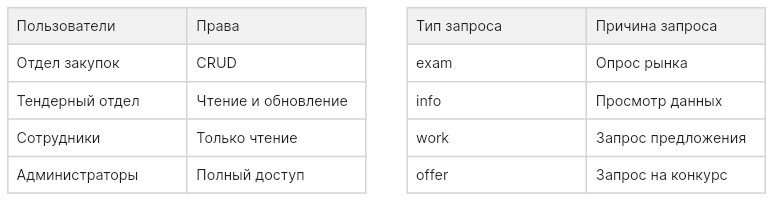
\includegraphics[width=6in]{schem.png}

\section*{Реализация}
Можно ознакомиться с первой версией и начать корректировать вектор развития, архитектура представляет из себя часть отвечающую за обработку запросов и часть хранящую данные. API Swagger для просмотра эндпоинтов:

\begin{center}
    http://185.244.172.177:3000/api/docs
\end{center}

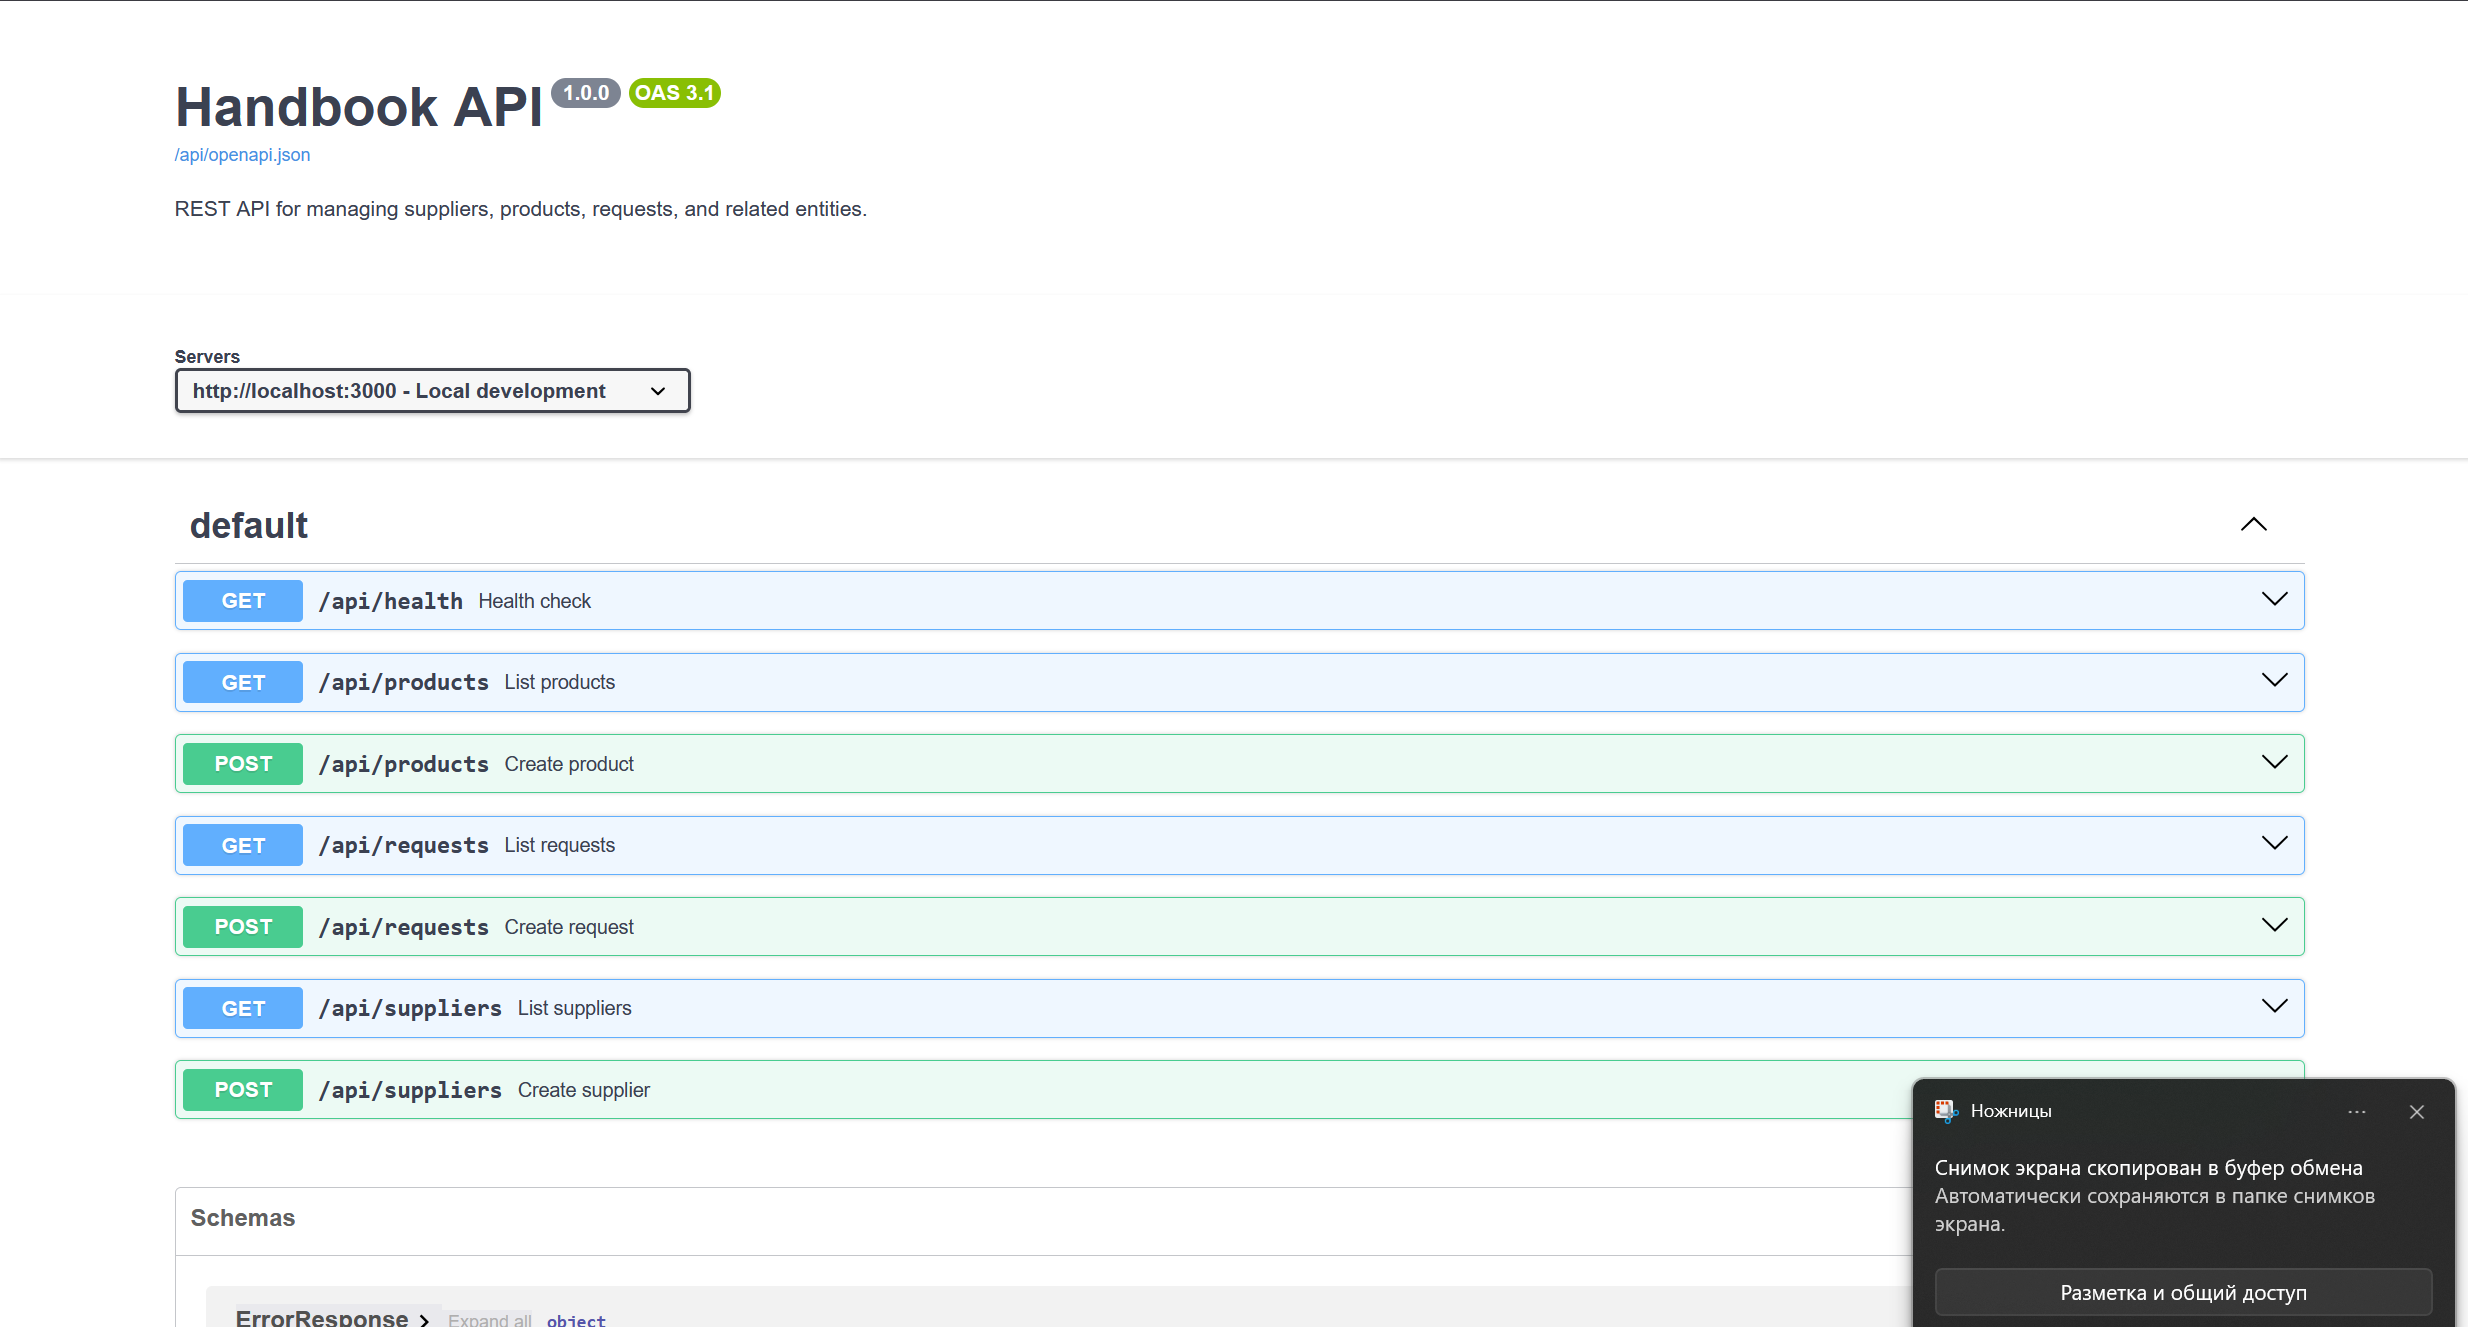
\includegraphics[width=6in]{swagger.png}

\newpage
\section*{Взаимодействие}
Для визуального представления работы системы был разработан временный интерфейс, в котором можно посмотреть все функции доступные на данный момент:

\begin{center}
    http://185.244.172.177:3000
\end{center}

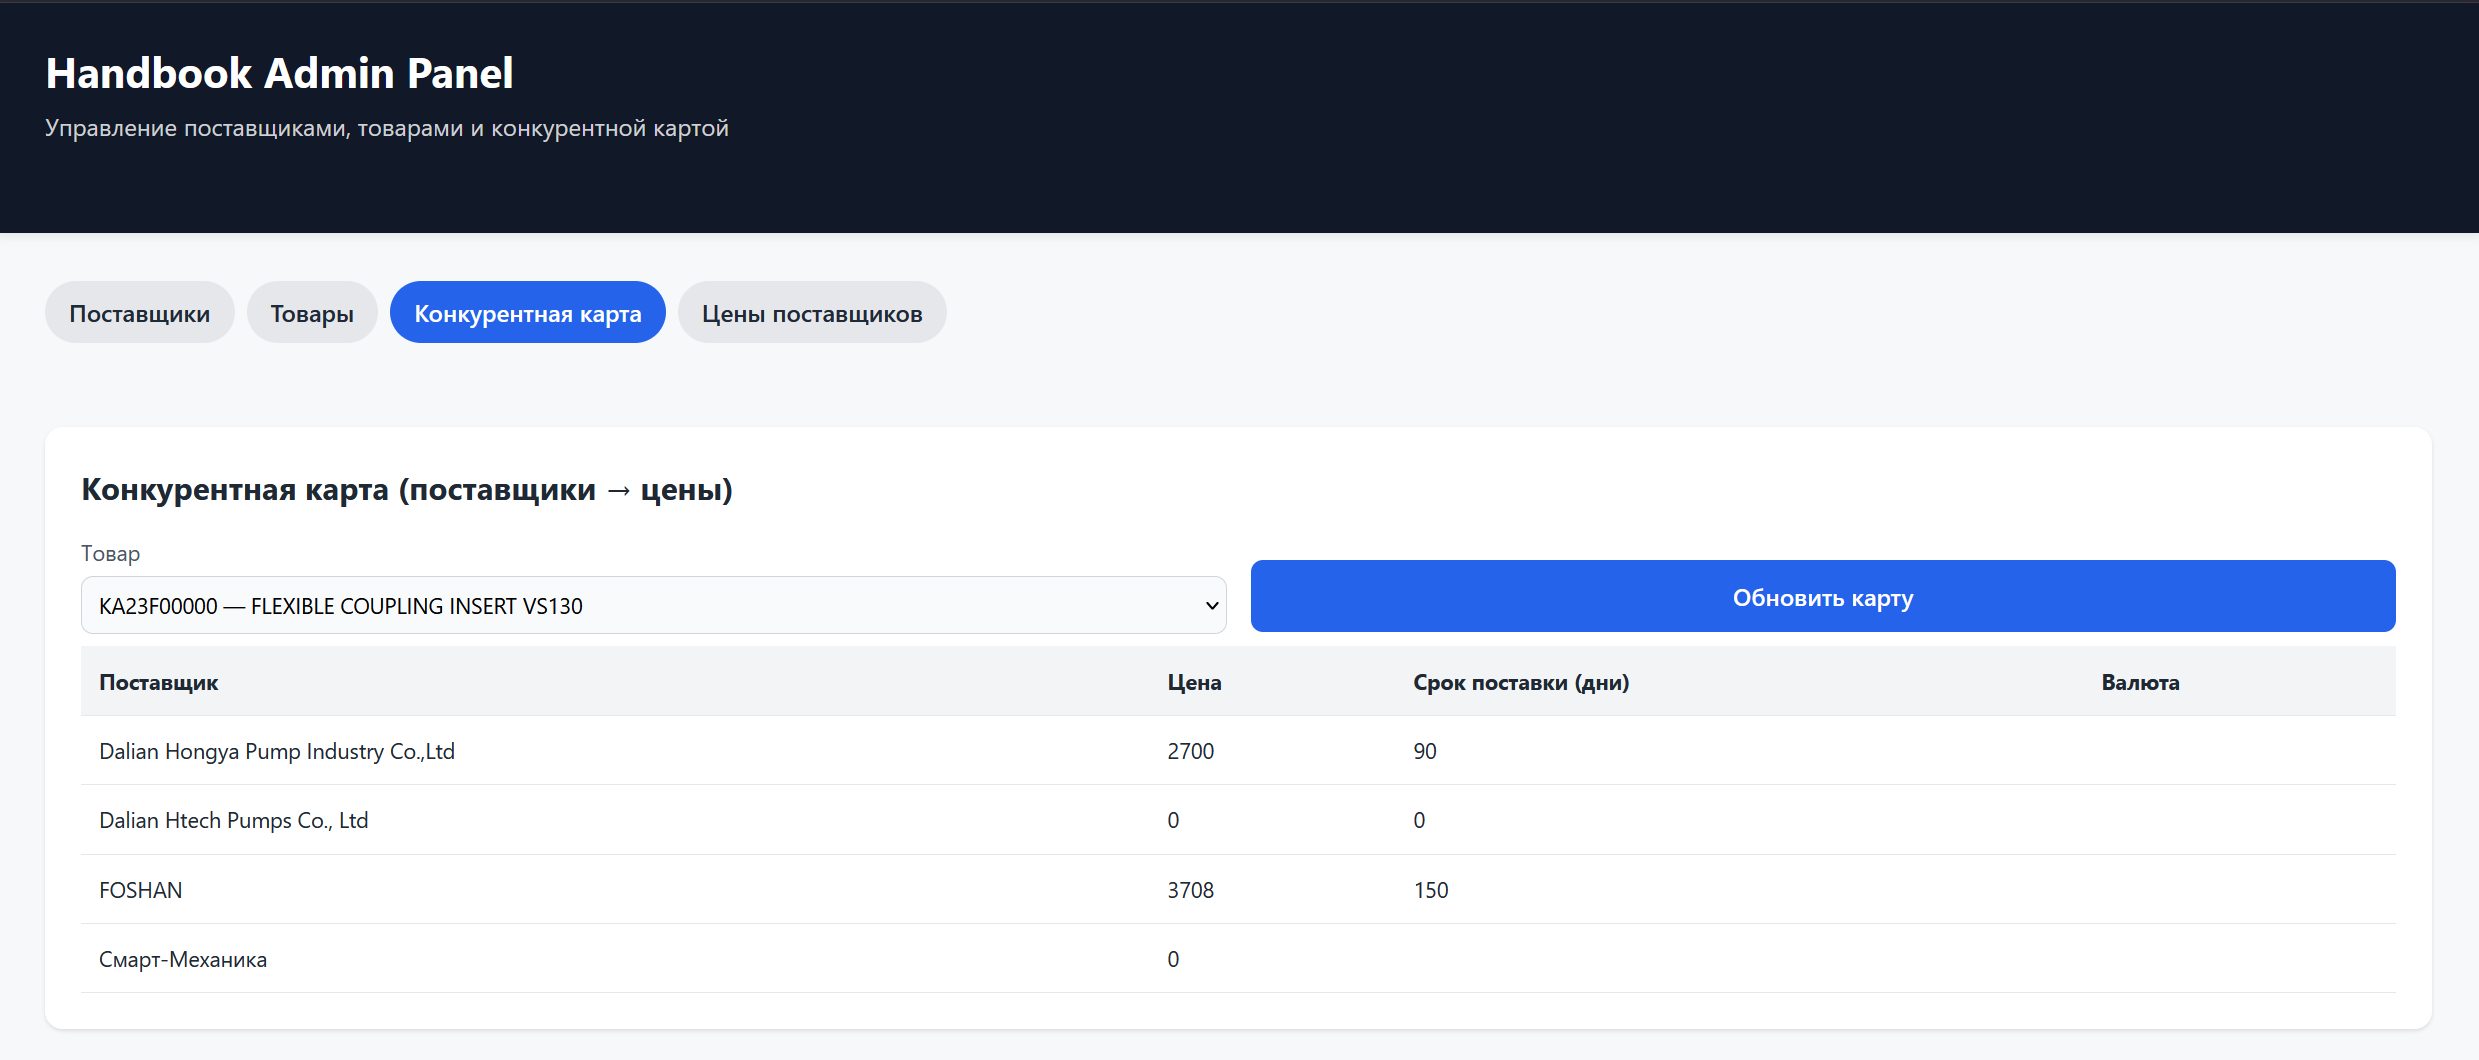
\includegraphics[width=6in]{screen_page.png}

\section*{В планах}
Изучение инструментов битрикса для интеграции решения, исправление некорретности работы системы, если таковые будут выявлены, добавление функций улучшающих пользовательское взаимодействие или фич.

\end{document}